
\documentclass[english]{article}
\usepackage[T1]{fontenc}
\usepackage[latin9]{inputenc}
\usepackage{float}
\usepackage{url}
\usepackage{amsmath}
\usepackage{amssymb}
\usepackage{stackrel}
\usepackage{graphicx}

\makeatletter


\usepackage[dvipsnames,table]{xcolor}

\usepackage{lineno}
\linenumbers
\linespread{1.25}

\usepackage{longtable}
\usepackage{pdflscape}

\usepackage[bookmarks=true]{hyperref}
\usepackage{orcidlink}
\usepackage{booktabs}
\usepackage{caption}
\usepackage{longtable}
% \usepackage[T1]{fontenc}
\usepackage{geometry}
\geometry{verbose,tmargin=2cm,bmargin=2cm,lmargin=2cm,rmargin=2cm}
\usepackage{array}
\usepackage{url}
\usepackage{multirow}
\usepackage{stackrel}
\usepackage{rotating}

\usepackage{bbold}


\usepackage{array} % for ExtraRowHeight

\usepackage{graphicx}
\usepackage{siunitx}
\usepackage[normalem]{ulem}
\usepackage{colortbl}

\usepackage{hhline}
\usepackage{calc}
\usepackage{tabularx}
\usepackage{threeparttable}
\usepackage{wrapfig}
\usepackage{adjustbox}


\usepackage{hyperref}

\newcolumntype{L}{>{\raggedright\arraybackslash}}
\newcolumntype{R}{>{\raggedleft\arraybackslash}}
\newcolumntype{C}{>{\centering\arraybackslash}}

% \renewcommand{\arraystretch}{1.5}
\renewcommand{\tabcolsep}{0.2cm}

\setlength{\LTpre}{6pt}
\setlength{\LTpost}{6pt}

\makeatother

\usepackage{babel}





% https://tex.stackexchange.com/questions/151241/remove-metadata-of-pdf-generated-by-latex
\hypersetup{
    bookmarks=true,         % show bookmarks bar?
    unicode=false,          % non-Latin characters in Acrobat's bookmarks
    pdftoolbar=true,        % show Acrobat's toolbar?
    pdfmenubar=true,        % show Acrobat's menu?
    pdffitwindow=false,     % window fit to page when opened
%    pdfstartview={FitW},    % fits the width of the page to the window
    pdftitle={Defeating a Black Marble Flood Against Monero: Best Options for Ring Size and Transaction Fee},    % title
    pdfauthor={Rucknium},     % author
    pdfsubject={},   % subject of the document
    pdfcreator={Rucknium},   % creator of the document
    pdfproducer={},  % producer of the document
    pdfkeywords={}, % list of keywords
    pdfnewwindow=true,      % links in new window
    colorlinks=false,       % false: boxed links; true: colored links
    linkcolor=red,          % color of internal links
    citecolor=green,        % color of links to bibliography
    filecolor=magenta,      % color of file links
    urlcolor=cyan           % color of external links
}




\begin{document}

\title{Defeating a Black Marble Flood Against Monero: Best Options for Ring Size and Transaction Fee\\\vspace{.3cm}
\large Draft v0.1\vspace{-.715cm}}
\author{Rucknium\orcidlink{0000-0001-5999-8950} }
\date{May 28, 2024}




\maketitle

\section{Summary}

Increasing Monero's ring size and minimum transaction fee are two
options for defeating black marble flooding. This document attempts
to answer the question: Is it better to increase the ring size or
the transaction fee, or some combination of the two? Cost-Effectiveness
Analysis is used to analyze this question. It considers the additional
costs imposed on transacting users and node operators compared to
the benefit of stronger resistance to black marble flooding.

Consider an adversary with a daily budget of 12.5 XMR, five times
higher than the daily expenditure of the suspected March 2024 black
marble flooder. Given the constraints considered, the most cost-effective
combination of defense parameters are ring size 60 and minimum 70
nanonero per byte fee. Effective ring size would be 22.8 if the adversary
spent his entire budget every day. The 2in/2out reference transaction
with ring size 60 would be about 140\% larger than the transaction
with current ring size 16. The user's cost to send this transaction
would be about 4.4 USD cents. The total time to verify all transactions
in a block of normal transaction volume would increase from 0.5 seconds
to 1.8 seconds. An unpruned node would grow 59 GB in a year instead
of 25 GB. Pruned nodes would grow 14 GB instead of 8 GB. 

\section{Black marble flooding as a game}

We will analyze the problem as a game with two players. One player
aims to flood the Monero blockchain with black marble outputs. This
player is limited by his budget. The other player aims to deter the
first player, or at least limit the damage, by choosing minimum fee
and ring size. This player is limited by the costs that fees and ring
size impose of transacting users and node operators.

Sam is a privacy adversary. His goal is to reduce Monero's effective
ring size by flooding the Monero blockchain with black marble outputs
that he owns. He has some budget $b$ denominated in XMR to spend
on transaction fees per block.

Alice wishes to defeat Sam. She can set Monero's ring size and minimum
transaction fee to try to accomplish her goal. Sam would have to spend
more XMR per output if the minimum fee per byte were higher. A larger
ring size would require Sam to own a larger share of outputs to achieve
a specified effective ring size. (Without changing the minimum fee
per byte, a larger ring size also requires Sam to spent more XMR to
produce each output because transaction size is larger.)

Larger ring sizes and fees help Alice accomplish her goal of defeating
Sam, but Alice cannot raise ring size and fee without limit. Users
who send Monero transactions need to pay a higher fee when the minimum
transaction fee is higher. Larger ring sizes mean that transactions
are larger. At a given transaction volume, larger transactions make
the blockchain grow faster. People who operate Monero nodes need to
store the blockchain on their storage media such as Solid State Drives
(SSDs). Alice needs to balance the benefit of greater defense against
Sam against the cost imposed on transacting users and node operators.

These are the factors on Alice's mind:
\begin{itemize}
\item I do not know Sam's budget $b$. I do not know what effective ring
size he hopes to achieve. If I set ring size and fee so that he cannot
achieve his desired effective ring size with his budget $b$, he will
choose not to flood the blockchain with black marbles. This is the
deterrence outcome.
\item If I fail to deter Sam, at least I can hold him to a specific effective
ring size when he spends his budget $b$. This is the fallback outcome.
\item I do not want to set ring size and transaction fee unnecessarily high
because transacting users and node operators pay higher costs when
these parameters increase.
\end{itemize}
We will simplify the problem:
\begin{itemize}
\item Sam may actually change the budget he is willing to spend based on
the effective ring size he is able to achieve. In other words, Sam
may have a tradeoff function between budget and effective ring size.
We will ignore this complication and assume that Sam's budget is fixed,
but unknown to Alice.
\item We will use the fallback outcome to measure the effectiveness of Alice's
options. When the fallback outcome is better for Alice, the deterrence
outcome is more likely. Therefore, it is a little redundant to compute
the probability of the deterrence outcome as an effectiveness metric.
\item Transaction volume by normal users is assumed to be constant and unaffected
by changes in the transaction fee. In other words, we will assume
that the demand for Monero transactions is completely inelastic with
respect to transaction fee.
\item We will assume that Sam's black marble transactions are 1in/2out because
the suspected black marble flood of March 2024 used this type of transaction.
Sam could produce black marble outputs more cheaply with 1in/16out
transactions, but the flood transactions would be easier for an observer
to identify.
\end{itemize}
Alice will use Cost-Effectiveness Analysis (CEA) to evaluate her ring
size and fee options. Cost effectiveness is the ratio of cost to effectiveness:

\begin{equation}
CE=\dfrac{\mathrm{Cost}}{\mathrm{Effectiveness}}
\end{equation}

A lower value of $CE$ is better. Alice must define cost and effectiveness
as functions of ring size, transaction fee, and the adversary's budget.
Let $n$ be nominal ring size, $f$ be the fee per byte in nanonero
units, and $b$ be the adversary's budget. Costs will be measured
in terms of XMR per block.

The cost has two components: cost to transacting users and cost to
node operators. The $i$th transaction has some number of inputs and
outputs. Changing the ring size $n$ changes the total size of the
$i$th transaction, which affects the total minimum fee to send the
transactions. And changing the minimum fee per byte changes the total
fee, of course. Let $w_{i}\left(n\right)$ be the weight of transaction
$i$ when ring size is $n$. When a transaction has two outputs, transaction
weight is equal to transaction size in bytes. Weight is larger than
size when the number of outputs is greater than two.\footnote{See Section 7.3.2 of koe, Alonso, K. M., \& Noether, S. (2020). \textit{Zero
to Monero: Second Edition}.} The block is assumed to contain an average set of transactions $T$.
The average is based on observed transactions confirmed on the blockchain
in the four weeks before the March 2024 suspected black marble flooding:
February 5 -- March 3. $C_{u}\left(f,n\right)$ is the aggregate
users' cost to send transactions for an average block:

\begin{equation}
C_{u}\left(f,n\right)=\underset{i\in T}{\sum}f\cdot w_{i}\left(n\right)
\end{equation}

The cost to node operators is a function of ring size. Node operators
do not pay higher costs when the minimum transaction fee is higher.
All units of computer storage in this document will be SI units, i.e.
a kilobyte, megabyte, gigabyte and terabyte are $10^{3}$, $10^{6}$,
$10^{9}$, and $10^{12}$ bytes, respectively. The retail price of
one consumer 1 TB SATA SSD is about 1 XMR.\footnote{In April 2024, the median retail price of a 1TB SATA SSD on \url{https://ssd.userbenchmark.com/}
was 114.50 USD. The exchange rate at the time was 120 USD per XMR.} A node operator's cost $C_{SSD}$ to store one byte of Monero blockchain
data is $10^{-12}$ XMR (a piconero). According to \texttt{monero.fail/map},
there were about 20,000 Monero nodes on the network in April 2024.
Currently the minimum relay fee is 20,000 piconeros (20 nanoneros)
per byte. Therefore, by coincidence Monero transactions pay for their
own storage space on the node network when users pay the minimum fee
per byte.

Let $d_{n}$, the number of nodes (daemons), be 20,000. $z_{i}\left(n\right)$
is the size of the $i$th transaction in the $T$ set when ring size
is $n$. The $m$ is an adjustment parameter that raises or lowers
total node operators' costs by a linear factor to adjust for uncertainty
about the true number of nodes and to add costs that are more difficult
to compute like CPU and RAM use. In the analysis below $m$ will be
set to 2. We will assume that each node is an unpruned node that stores
all transaction data in full. The total cost to node operators is
the sum of the size of transactions in the $T$ set multiplied by
the storage cost on a single SSD, the number of nodes on the network,
and the $m$ adjustment parameter:

\begin{equation}
C_{d}\left(n,m\right)=m\cdot d_{n}\cdot C_{SSD}\cdot\underset{i\in T}{\sum}z_{i}\left(n\right)
\end{equation}

Notice that $C_{d}\left(n,m\right)$ is the cost to node operators
under normal transaction volume, i.e. when there is no black marble
flooding. Total cost is the sum of $C_{u}\left(f,n\right)$ and $C_{d}\left(n,m\right)$:

\begin{equation}
C\left(f,n,m\right)=C_{u}\left(f,n\right)+C_{d}\left(n,m\right)
\end{equation}

With budget $b$, Sam can afford to place $\frac{b}{f}$ bytes of
transaction data in a block. Sam would create transactions with one
input and two outputs. The formula for the number of bytes of a transaction
like this in terms of the ring size $n$ is $975+35n$. The $975$
bytes is the size of the transaction except for the linear cost of
the ring size, i.e. a (invalid) 1in/2out transaction with ring size
0 would have $975$ bytes composed of the input's key image, other
input data that does not scale up with ring size, the outputs' bulletproofs+,
the outputs' public key, and \texttt{tx\_extra} data. The $35$ coefficient
on $n$ is the sum of the bytes of the ``$s$'' component of the
CLSAG ring signature of each ring member (32 bytes) and $3$ bytes
of the key offset integer that is used to create the output indices
of the ring members. The $3$ bytes is an empirical average of the
byes used by each key offset integer. The number of outputs per byte
that Sam produces is $2/\left(975+35n\right)$ because each of his
transaction has two outputs. To calculate the number of outputs per
block that Sam can afford with budget $b$ when fee is $f$ and nominal
ring size is $n$, we compute the product of $\frac{b}{f}$ and $2/\left(975+35n\right)$,
producing the formula for $s\left(b,f,n\right)$:

\begin{equation}
s\left(b,f,n\right)=\dfrac{2b}{f\cdot\left(975+35n\right)}
\end{equation}

Let $r$ be the number of real user outputs. When the number of outputs
owned by Sam is $s\left(b,f,n\right)$, the long-term mean effective
ring size\footnote{For a derivation of mean effective ring size, see Section 3 of Draft
v0.2 of Rucknium (2024) ``March 2024 Suspected Black Marble Flooding
Against Monero: Privacy, User Experience, and Countermeasures'' \url{https://github.com/Rucknium/misc-research/blob/main/Monero-Black-Marble-Flood/pdf/monero-black-marble-flood.pdf}} is

\begin{equation}
n_{e}\left(b,f,n\right)=1+\left(n-1\right)\cdot\dfrac{r}{r+s\left(b,f,n\right)}\label{eq:expectation-n_e}
\end{equation}

Alice wants to have a larger $n_{e}$ when Sam is producing black
marbles. $n_{e}$ is the desired outcome in the cost-effectiveness
analysis:

\begin{equation}
CE=\dfrac{C\left(f,n,m\right)}{n_{e}\left(b,f,n\right)}\label{eq:cost-effectiveness-full}
\end{equation}

Alice's goal is to choose minimum fee per byte $f$ and nominal ring
size $n$ to minimize $CE$ when Sam spends his budget $b$ producing
black marbles and the node cost multiplier is some specified $m$.
In game theory, a player's \textit{best response} in a two-player
game is a strategy that gives the player the best payoff when the
other player plays some specified strategy. Alice's best response
to Sam playing some $b$ as a strategy is to set $f$ and $n$ to
minimize $CE$. Alice does not know what value of $b$ Sam intends
to play, but reasonable values of $b$ can be analyzed to guide reasonable
choices of $f$ and $n$. In game theory terms, Alice's uncertainty
about Sam's $b$ means that this is a game of imperfect information.
Sam's player ``type'' is the unknown $b$. Sam has some probability
of being each type. In this document I will not explicitly declare
some probability distribution of Sam's type, but one could determine
Alice's single best response for the expected value of her cost effectiveness
when Sam's type has some probability distribution.

Define $f_{\min}$ and $f_{\max}$ as the minimum and maximum $f$
that Alice is willing to set. Let $n_{\min}$ and $n_{\max}$ be the
minimum and maximum $n$ that Alice is willing to set. Assume that
Alice wants to make sure that the effective ring size does not fall
below some specified minimum acceptable limit $\check{n}_{e}$. Alice
will try to minimize (\ref{eq:cost-effectiveness-full}) except when
the effective ring size would be below $\check{n}_{e}$ at the minimum
of (\ref{eq:cost-effectiveness-full}). In that case, Alice will exclude
the values of $n$ and $f$ that cause effective ring size to be below
$\check{n}_{e}$, then choose $n$ and $f$ to minimize (\ref{eq:cost-effectiveness-full})
from the set of $n$ and $f$ values that remain.

Alice's best response correspondence given Sam's choice of $b$ and
the node cost multiplier $m$ is the solution to

\begin{equation}
\begin{array}{l}
\underset{f,n}{\arg\min}\dfrac{C\left(f,n,m\right)}{n_{e}\left(b,f,n\right)}\\
\mathrm{subject\,to}\\
f_{\min}\leq f,\,f\leq f_{\max}\\
n_{\min}\leq n,\,n\leq n_{\max}\\
\check{n}_{e}\leq n_{e}\left(b,f,n\right)
\end{array}\label{eq:best-response-correspondence}
\end{equation}

The problem in (\ref{eq:best-response-correspondence}) is a nonlinear
minimization problem with nonlinear inequality constraints. Note that
the constraint set is convex, but the objective function is neither
globally convex nor globally concave.\footnote{The full proof of this statement is TODO. The first four constraints
form a convex set because they are affine. The $\check{n}_{e}\leq n_{e}\left(b,f,n\right)$
constraint is more complicated. The Hessian matrix of the second-order
partial derivatives of $n_{e}$ with respect to $f$ and $n$ is negative
definite as long as $n>1$. That means that its superlevel set for
some $\check{n}_{e}$ is convex. (The $\check{n}_{e}\leq n_{e}\left(b,f,n\right)$
inequality defines the superlevel set.) The intersection of two convex
sets is convex, so the constraint set of (\ref{eq:best-response-correspondence})
is convex.} The necessary conditions for the solution could be found analytically
by checking the Karush-Kuhn-Tucker conditions. I will solve it numerically
with a grid search. The grid is formed by evaluating (\ref{eq:cost-effectiveness-full})
many times at different values of $f$ and $n$. The values of $f$
are 40 equally-spaced values between $f_{\min}$ and $f_{\max}$.
The values of $n$ are each integer between $n_{\min}$ and $n_{\max}$.

We will start with a simple example. Assume that the adversary's budget
is 2.5 XMR per day. This is approximately the expenditure rate of
the suspected black marble flooder in March 2024. We will evaluate
cost-effectiveness at each combination of $f=\left\{ 10,20,40,100,200\right\} $
nanoneros per byte and $n=\left\{ 16,30,45,60\right\} $ ring size.

Table \ref{table-2_5-budget} contains the cost effectiveness (CE)
computations with other metrics like transaction size, total projected
growth of the blockchain, and estimated transaction verification time.
Note that the cost to send a 2in/2out transaction increases when ring
size increases even if the fee per byte does not increase because
users have to pay for larger total transaction size. The numerator
of CE has been scaled to millineros. The lowest value in the CE column
is 0.48 when nominal ring size is 60 and minimum fee is 40 nanoneros
per byte. Sam can achieve a 37.5 effective ring size with a 2.5 XMR/day
budget when nominal ring size is 60 and minimum fee is 40 nanoneros
per byte. Estimation of transaction and block verification time is
explained in Appendix \ref{sec:Appendix:-Transaction-verification}..

Figure \ref{fig-contour-plot-50-budget} is a shaded contour plot
of cost effectiveness when Sam has a budget of 50 XMR per day. Lighter
colors on the plot indicate lower CE values at the specified minimum
fee and ring size values. The blue triangle indicates the fee and
ring size values that minimize the CE when the minimum acceptable
effective ring size of 5 is disregarded. When we allow only fee and
ring size values that produce effective ring size above the minimum
acceptable effective ring, the green circle indicates the fee and
ring size values that minimize the CE. In this plot the triangle and
circle are at the same location because the minimum CE produces an
effective ring size of 12.8, above the minimum effective ring size
of 5. 

Table \ref{table-scenarios-budget} shows the values of minimum fee
and ring size that produce optimal cost effectiveness when Sam has
different budgets. The maximum budget, 500 XMR per day, exceeds Monero's
daily security budget provided by tail emission. An adversary's budget
higher than 500 might imply that the adversary could directly 51 percent
attack the blockchain by renting CPU hashpower. It seems unnecessary
to consider a black marble flooder's budget greater than 500 XMR per
day because an adversary with a higher budget might be able to do
more damage to Monero than flooding the blockchain with black marble
outputs.

\begin{landscape}
\footnotesize{
\setlength{\LTpost}{0mm}
\begin{longtable}{Rp{1.75cm}Rp{1cm}Rp{1.5cm}Rp{0.75cm}Rp{1cm}Rp{2cm}Rp{1.5cm}Rp{0.75cm}Rp{1.4cm}Rp{1cm}Rp{1cm}Rp{1cm}Rp{1cm}Rp{1cm}Rp{0.75cm}Rp{1.4cm}}
\caption{
{\large Cost effectiveness of minimum fee and ring size options when adversary budget is 2.5 XMR per day}
} \\ 
\toprule
 &  &  &  &  &  &  & \multicolumn{4}{c}{Normal tx volume} & \multicolumn{5}{c}{Normal tx volume + black marble flooding} \\ 
\cmidrule(lr){8-11} \cmidrule(lr){12-16}
 &  &  &  &  &  &  &  &  & \multicolumn{4}{c}{One year blockchain growth (GB)} &  &  &  \\ 
\cmidrule(lr){10-13}
Adversary XMR budget per day & Nominal ring size & Min fee (nanoneros per byte) & CE & Size of 2in/2out (bytes) & User's cost to send 2in/2out (USD cents) & Seconds to verify 2in/2out & Block size (KB) & Seconds to verify txs in block & Unpruned & Pruned & Unpruned & Pruned & Effective ring size & Block size (KB) & Seconds to verify txs in block \\ 
\midrule\addlinespace[2.5pt]
$2.50$ & 16 & $10$ & $1.36$ & $2,219$ & $0.27$ & $0.012$ & $95$ & $0.54$ & $25$ & $8$ & $116$ & $34$ & $3.59$ & $443$ & $2.69$ \\ 
\cellcolor[HTML]{00FF00}{\textcolor[HTML]{000000}{$2.50$}} & \cellcolor[HTML]{00FF00}{\textcolor[HTML]{000000}{16}} & \cellcolor[HTML]{00FF00}{\textcolor[HTML]{000000}{$20$}} & \cellcolor[HTML]{00FF00}{\textcolor[HTML]{000000}{$1.08$}} & \cellcolor[HTML]{00FF00}{\textcolor[HTML]{000000}{$2,219$}} & \cellcolor[HTML]{00FF00}{\textcolor[HTML]{000000}{$0.53$}} & \cellcolor[HTML]{00FF00}{\textcolor[HTML]{000000}{$0.012$}} & \cellcolor[HTML]{00FF00}{\textcolor[HTML]{000000}{$95$}} & \cellcolor[HTML]{00FF00}{\textcolor[HTML]{000000}{$0.54$}} & \cellcolor[HTML]{00FF00}{\textcolor[HTML]{000000}{$25$}} & \cellcolor[HTML]{00FF00}{\textcolor[HTML]{000000}{$8$}} & \cellcolor[HTML]{00FF00}{\textcolor[HTML]{000000}{$71$}} & \cellcolor[HTML]{00FF00}{\textcolor[HTML]{000000}{$21$}} & \cellcolor[HTML]{00FF00}{\textcolor[HTML]{000000}{$5.41$}} & \cellcolor[HTML]{00FF00}{\textcolor[HTML]{000000}{$269$}} & \cellcolor[HTML]{00FF00}{\textcolor[HTML]{000000}{$1.62$}} \\ 
$2.50$ & 16 & $40$ & $0.99$ & $2,219$ & $1.07$ & $0.012$ & $95$ & $0.54$ & $25$ & $8$ & $48$ & $14$ & $7.82$ & $182$ & $1.08$ \\ 
$2.50$ & 16 & $100$ & $1.21$ & $2,219$ & $2.66$ & $0.012$ & $95$ & $0.54$ & $25$ & $8$ & $34$ & $10$ & $11.14$ & $130$ & $0.75$ \\ 
$2.50$ & 16 & $200$ & $1.75$ & $2,219$ & $5.33$ & $0.012$ & $95$ & $0.54$ & $25$ & $8$ & $30$ & $9$ & $13.10$ & $113$ & $0.64$ \\ 
$2.50$ & 30 & $10$ & $0.97$ & $3,196$ & $0.38$ & $0.022$ & $136$ & $0.94$ & $36$ & $10$ & $127$ & $34$ & $7.25$ & $483$ & $3.82$ \\ 
$2.50$ & 30 & $20$ & $0.74$ & $3,196$ & $0.77$ & $0.022$ & $136$ & $0.94$ & $36$ & $10$ & $81$ & $22$ & $11.29$ & $310$ & $2.38$ \\ 
$2.50$ & 30 & $40$ & $0.69$ & $3,196$ & $1.53$ & $0.022$ & $136$ & $0.94$ & $36$ & $10$ & $59$ & $16$ & $16.19$ & $223$ & $1.66$ \\ 
$2.50$ & 30 & $100$ & $0.87$ & $3,196$ & $3.83$ & $0.022$ & $136$ & $0.94$ & $36$ & $10$ & $45$ & $12$ & $22.26$ & $171$ & $1.23$ \\ 
$2.50$ & 30 & $200$ & $1.29$ & $3,196$ & $7.67$ & $0.022$ & $136$ & $0.94$ & $36$ & $10$ & $40$ & $11$ & $25.54$ & $153$ & $1.09$ \\ 
$2.50$ & 45 & $10$ & $0.76$ & $4,242$ & $0.51$ & $0.032$ & $180$ & $1.38$ & $47$ & $12$ & $138$ & $35$ & $12.31$ & $527$ & $4.68$ \\ 
$2.50$ & 45 & $20$ & $0.59$ & $4,242$ & $1.02$ & $0.032$ & $180$ & $1.38$ & $47$ & $12$ & $93$ & $24$ & $19.00$ & $353$ & $3.03$ \\ 
$2.50$ & 45 & $40$ & $0.56$ & $4,242$ & $2.04$ & $0.032$ & $180$ & $1.38$ & $47$ & $12$ & $70$ & $18$ & $26.55$ & $267$ & $2.21$ \\ 
$2.50$ & 45 & $100$ & $0.73$ & $4,242$ & $5.09$ & $0.032$ & $180$ & $1.38$ & $47$ & $12$ & $56$ & $15$ & $35.14$ & $215$ & $1.71$ \\ 
$2.50$ & 45 & $200$ & $1.10$ & $4,242$ & $10.18$ & $0.032$ & $180$ & $1.38$ & $47$ & $12$ & $52$ & $13$ & $39.45$ & $197$ & $1.55$ \\ 
$2.50$ & 60 & $10$ & $0.63$ & $5,289$ & $0.63$ & $0.043$ & $223$ & $1.82$ & $59$ & $14$ & $150$ & $37$ & $18.37$ & $571$ & $5.39$ \\ 
$2.50$ & 60 & $20$ & $0.50$ & $5,289$ & $1.27$ & $0.043$ & $223$ & $1.82$ & $59$ & $14$ & $104$ & $26$ & $27.84$ & $397$ & $3.60$ \\ 
\cellcolor[HTML]{FFA500}{\textcolor[HTML]{000000}{$2.50$}} & \cellcolor[HTML]{FFA500}{\textcolor[HTML]{000000}{60}} & \cellcolor[HTML]{FFA500}{\textcolor[HTML]{000000}{$40$}} & \cellcolor[HTML]{FFA500}{\textcolor[HTML]{000000}{$0.48$}} & \cellcolor[HTML]{FFA500}{\textcolor[HTML]{000000}{$5,289$}} & \cellcolor[HTML]{FFA500}{\textcolor[HTML]{000000}{$2.54$}} & \cellcolor[HTML]{FFA500}{\textcolor[HTML]{000000}{$0.043$}} & \cellcolor[HTML]{FFA500}{\textcolor[HTML]{000000}{$223$}} & \cellcolor[HTML]{FFA500}{\textcolor[HTML]{000000}{$1.82$}} & \cellcolor[HTML]{FFA500}{\textcolor[HTML]{000000}{$59$}} & \cellcolor[HTML]{FFA500}{\textcolor[HTML]{000000}{$14$}} & \cellcolor[HTML]{FFA500}{\textcolor[HTML]{000000}{$82$}} & \cellcolor[HTML]{FFA500}{\textcolor[HTML]{000000}{$20$}} & \cellcolor[HTML]{FFA500}{\textcolor[HTML]{000000}{$37.90$}} & \cellcolor[HTML]{FFA500}{\textcolor[HTML]{000000}{$310$}} & \cellcolor[HTML]{FFA500}{\textcolor[HTML]{000000}{$2.71$}} \\ 
$2.50$ & 60 & $100$ & $0.65$ & $5,289$ & $6.35$ & $0.043$ & $223$ & $1.82$ & $59$ & $14$ & $68$ & $17$ & $48.60$ & $258$ & $2.18$ \\ 
$2.50$ & 60 & $200$ & $1.01$ & $5,289$ & $12.69$ & $0.043$ & $223$ & $1.82$ & $59$ & $14$ & $63$ & $16$ & $53.69$ & $241$ & $2.00$ \\ 
\bottomrule
\label{table-2_5-budget}
\end{longtable}
\begin{minipage}{\linewidth}
Row in green is the status quo. Row in orange is the best cost effectiveness.\\
\end{minipage}

}
\end{landscape}

\begin{figure}
\caption{Most cost-effective minimum fee and ring size when adversary budget
is 50 XMR per day}

\label{fig-contour-plot-50-budget}

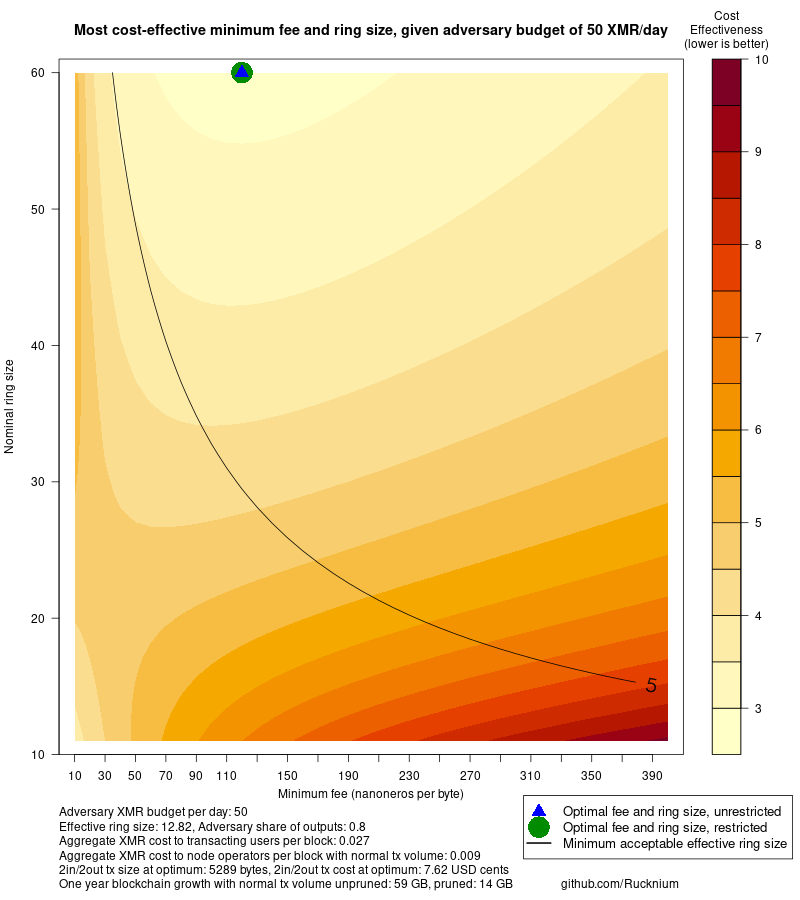
\includegraphics[scale=0.65]{images/cost-effective-contour-plot-50-budget}
\end{figure}

\begin{landscape}
\footnotesize{
\setlength{\LTpost}{0mm}
\begin{longtable}{Rp{1.75cm}Rp{1cm}Rp{1.5cm}Rp{0.75cm}Rp{1cm}Rp{2cm}Rp{1.5cm}Rp{0.75cm}Rp{1.4cm}Rp{1cm}Rp{1cm}Rp{1cm}Rp{1cm}Rp{1cm}Rp{0.75cm}Rp{1.4cm}}
\caption{
{\large Minimum fee and ring size at optimal cost effectiveness, adversary budget scenarios}
} \\ 
\toprule
 &  &  &  &  &  &  & \multicolumn{4}{c}{Normal tx volume} & \multicolumn{5}{c}{Normal tx volume + black marble flooding} \\ 
\cmidrule(lr){8-11} \cmidrule(lr){12-16}
 &  &  &  &  &  &  &  &  & \multicolumn{4}{c}{One year blockchain growth (GB)} &  &  &  \\ 
\cmidrule(lr){10-13}
Adversary XMR budget per day & Nominal ring size & Min fee (nanoneros per byte) & CE & Size of 2in/2out (bytes) & User's cost to send 2in/2out (USD cents) & Seconds to verify 2in/2out & Block size (KB) & Seconds to verify txs in block & Unpruned & Pruned & Unpruned & Pruned & Effective ring size & Block size (KB) & Seconds to verify txs in block \\ 
\midrule\addlinespace[2.5pt]
\cellcolor[HTML]{00FF00}{\textcolor[HTML]{000000}{$2.50$}} & \cellcolor[HTML]{00FF00}{\textcolor[HTML]{000000}{16}} & \cellcolor[HTML]{00FF00}{\textcolor[HTML]{000000}{$20$}} & \cellcolor[HTML]{00FF00}{\textcolor[HTML]{000000}{$1.08$}} & \cellcolor[HTML]{00FF00}{\textcolor[HTML]{000000}{$2,219$}} & \cellcolor[HTML]{00FF00}{\textcolor[HTML]{000000}{$0.53$}} & \cellcolor[HTML]{00FF00}{\textcolor[HTML]{000000}{$0.012$}} & \cellcolor[HTML]{00FF00}{\textcolor[HTML]{000000}{$95$}} & \cellcolor[HTML]{00FF00}{\textcolor[HTML]{000000}{$0.54$}} & \cellcolor[HTML]{00FF00}{\textcolor[HTML]{000000}{$25$}} & \cellcolor[HTML]{00FF00}{\textcolor[HTML]{000000}{$8$}} & \cellcolor[HTML]{00FF00}{\textcolor[HTML]{000000}{$71$}} & \cellcolor[HTML]{00FF00}{\textcolor[HTML]{000000}{$21$}} & \cellcolor[HTML]{00FF00}{\textcolor[HTML]{000000}{$5.41$}} & \cellcolor[HTML]{00FF00}{\textcolor[HTML]{000000}{$269$}} & \cellcolor[HTML]{00FF00}{\textcolor[HTML]{000000}{$1.62$}} \\ 
$0.25$ & 60 & $10$ & $0.24$ & $5,289$ & $0.63$ & $0.043$ & $223$ & $1.82$ & $59$ & $14$ & $68$ & $17$ & $48.60$ & $258$ & $2.18$ \\ 
$0.50$ & 60 & $10$ & $0.29$ & $5,289$ & $0.63$ & $0.043$ & $223$ & $1.82$ & $59$ & $14$ & $77$ & $19$ & $40.89$ & $293$ & $2.53$ \\ 
$1.25$ & 60 & $20$ & $0.37$ & $5,289$ & $1.27$ & $0.043$ & $223$ & $1.82$ & $59$ & $14$ & $82$ & $20$ & $37.90$ & $310$ & $2.71$ \\ 
$2.50$ & 60 & $30$ & $0.48$ & $5,289$ & $1.90$ & $0.043$ & $223$ & $1.82$ & $59$ & $14$ & $89$ & $22$ & $33.80$ & $339$ & $3.01$ \\ 
$5.00$ & 60 & $40$ & $0.66$ & $5,289$ & $2.54$ & $0.043$ & $223$ & $1.82$ & $59$ & $14$ & $104$ & $26$ & $27.84$ & $397$ & $3.60$ \\ 
$12.50$ & 60 & $70$ & $1.10$ & $5,289$ & $4.44$ & $0.043$ & $223$ & $1.82$ & $59$ & $14$ & $124$ & $30$ & $22.76$ & $471$ & $4.37$ \\ 
$25.00$ & 60 & $90$ & $1.73$ & $5,289$ & $5.71$ & $0.043$ & $223$ & $1.82$ & $59$ & $14$ & $160$ & $39$ & $17.11$ & $609$ & $5.78$ \\ 
$50.00$ & 60 & $120$ & $2.83$ & $5,289$ & $7.62$ & $0.043$ & $223$ & $1.82$ & $59$ & $14$ & $211$ & $52$ & $12.82$ & $802$ & $7.77$ \\ 
$125.00$ & 60 & $140$ & $5.68$ & $5,289$ & $8.89$ & $0.043$ & $223$ & $1.82$ & $59$ & $14$ & $385$ & $94$ & $7.17$ & $1,464$ & $14.56$ \\ 
$250.00$ & 60 & $180$ & $9.69$ & $5,289$ & $11.42$ & $0.043$ & $223$ & $1.82$ & $59$ & $14$ & $566$ & $138$ & $5.12$ & $2,152$ & $21.64$ \\ 
$500.00$ & 60 & $350$ & $17.47$ & $5,289$ & $22.21$ & $0.043$ & $223$ & $1.82$ & $59$ & $14$ & $580$ & $142$ & $5.02$ & $2,208$ & $22.20$ \\ 
\bottomrule
\label{table-scenarios-budget}
\end{longtable}
\begin{minipage}{\linewidth}
Row in green is the status quo\\
\end{minipage}

}
\end{landscape}

\section{Discussion}

What have we learned? According to this analysis, raising the ring
size is a more cost-effective strategy against a black marble
attack than raising fees. A combination of a large increase in ring
size and a modest increase in fee seems to provide a good, cost-effective
defense.

Consider an adversary with a daily budget of 12.5 XMR, five times
higher than the daily expenditure of the suspected March 2024 black
marble flooder. Table \ref{table-scenarios-budget} says the most
cost-effective combination of defense parameters are ring size 60
and minimum 70 nanonero per byte fee. Effective ring size would be
22.8 if Sam spent his entire budget every day. The 2in/2out reference
transaction with ring size 60 would be about 140\% larger than the
transaction with current ring size 16. The user's cost to send this
transaction would be about 4.4 USD cents. The total time to verify
all transactions in a block of normal transaction volume would increase
from 0.5 seconds to 1.8 seconds. An unpruned node would grow 59 GB
in a year instead of 25 GB. Pruned nodes would grow 14 GB instead
of 8 GB. 

Put these storage requirements into perspective. Recall that we use
base-10 (SI) units to measure bytes in this document. As of May 2024,
a unpruned Monero blockchain is 206 GB. A pruned Monero node takes
79 GB of storage space. The 2023 Ultra 4K edition of Call of Duty
requires 229 GB of storage.\footnote{{\scriptsize{}\url{https://web.archive.org/web/20231214215231/https://www.callofduty.com/blog/2023/10/call-of-duty-modern-warfare-III-specs-preloading-pc-trailer}}}
An unpruned BTC node requires 650 GB of storage and grows about 89
GB per year.\footnote{\url{https://bitcoin.stackexchange.com/a/116350} and \url{https://transactionfee.info/charts/block-size/}}
Therefore, with ring size 60 the Monero blockchain would grow slower
than the BTC blockchain, crossing the Call of Duty storage threshold
within a year.

Encouraging node operators to prune their nodes and implementing a
coinbase consolidation transaction type could reduce the impact of
increasing the minimum fee and ring size. Pruning could be encouraged
by setting pruning as the default in more Monero software interfaces,
such as the Monero GUI wallet Pull Request \#4320, and public information
campaigns.\footnote{\url{https://github.com/monero-project/monero-gui/pull/4320}}
A coinbase consolidation type would reduce the transaction size for
small coinbase outputs.\footnote{\url{https://github.com/monero-project/research-lab/issues/108}}

\section{Summary: Downsides and benefits of options}
\begin{enumerate}
\item Increase the minimum relay fee per byte
\begin{enumerate}
\item Downsides:
\begin{enumerate}
\item Users may make fewer transactions. That would reduce Monero's total
anonymity set because the rate of creation of new outputs would fall.
\item Users could move to another means of payment.
\item Monero might lose its reputation as a low-cost means of payment.
\item Large changes in Monero's fiat exchange rate could make the purchasing
power of the minimum fee much higher or lower than anticipated.
\end{enumerate}
\item Benefits:
\begin{enumerate}
\item Miners would earn more from fees. This would increase Monero's resistance
to 51 percent attack because its mining security budget would increase
a little.
\item Higher fees would increase the cost of all spam regardless of motivation.
(Increasing the ring size only negatively affects spammers that want
to reduce the effective ring size.)
\end{enumerate}
\end{enumerate}
\item Increase the ring size
\begin{enumerate}
\item Downsides:
\begin{enumerate}
\item Greater storage requirements for operating a Monero node could cause
some node operators to stop running their nodes. This would make the
Monero network less decentralized.
\item Some Monero wallet users may stop running local nodes and switch to
remote nodes. This would increase the load on public remote nodes
and potentially expose the wallet users to some privacy risks from
malicious remote nodes.\footnote{See \url{https://docs.featherwallet.org/guides/nodes}}
\item Verification time per transaction would increase. During normal operation,
the Monero node would use more CPU resources. During initial blockchain
download, total sync time would be greater. Syncing a Monero node
on a HDD, which is already very difficult, might become completely
nonviable because of the necessary random reads for ring signature
verification.
\item At extremes, long verification times can threaten network stability.
In 2023 Pirate Chain suffered a transaction spam attack that caused
chain splits because of long transaction verification times.\footnote{\url{https://web.archive.org/web/20230803171107/https://old.reddit.com/user/SignificantRoof5656/comments/15h9reh/pirate_chains_045_spam_attack_2_months_later/}}
Monero uses the Fluffy Blocks protocol to verify transactions as they
arrive in the txpool instead of bottlenecking verification at the
time new blocks are mined. It is unclear if Pirate Chain, a code fork
of Zcash, uses a compact block protocol.\footnote{See \url{https://github.com/zcash/zips/issues/360}}
As long as the time to verify each block's transactions does not become
a large fraction of mean time between blocks (120 seconds), this is
probably not a threatening issue, \textit{in theory}. In practice,
the Monero node performs many more actions than just verifying the
cryptography of transactions. There may be hidden bottlenecks. Recently,
spikes of transactions with large numbers of inputs have seemed to
cause excess RAM usage of nodes, shutting down nodes in some cases.\footnote{\url{https://github.com/monero-project/monero/issues/9317}}
\end{enumerate}
\item Benefits:
\begin{enumerate}
\item Increasing the ring size increases the anonymity set of all transaction
inputs. Other statistical attacks unrelated to black marble flooding
like EAE attacks and timing analysis would become more difficult.
\end{enumerate}
\item Neutral:
\begin{enumerate}
\item Increasing the ring size has very little effect on wallet sync times.
The bandwidth costs for syncing transactions in mined blocks are only
about three bytes per ring member for the ring offset data. No additional
computation is required. However, ring signature data is sent from
nodes to wallets when transactions are still in the txpool.\footnote{Thanks to jeffro256 for explaining this.}
\end{enumerate}
\end{enumerate}
\item Encourage blockchain pruning
\begin{enumerate}
\item Downsides:
\begin{enumerate}
\item New unpruned nodes may have to connect to more nodes to create an
unpruned copy of the blockchain.
\item All pruned nodes keep one-eighth of the transaction data that is designated
``prunable''. If all nodes on the network are pruned, there is an
extremely small chance that one of the eight pruning slices will not
exist on the whole network. That would mean that not all signature
data on the blockchain could be verified. When blockchain pruning
is enabled, a Monero node randomly chooses one of eight possible pruning
seeds independently of the pruning seeds that other nodes have chosen.
By chance, the network could be missing one of the eight slices of
the pruneable part of the blockchain because the choice of pruning
seed is not coordinated between nodes. This chance is extremely small.
If the network only has pruned nodes and the total number of nodes
on the network is 681, the probability of missing one of the eight
pruning slices is less than $2^{-128}$, which is the probability
of guessing a specific 12-word BIP39 bitcoin seed phrase with a single
guess. See Appendix \ref{sec:Probability-of-recovering-complete-blockchain-data}
for how to compute this probability. This probability does not consider
the challenge of new nodes finding their pruning slices by connecting
to multiple nodes throughout the network.
\end{enumerate}
\item Benefits:
\begin{enumerate}
\item Pruned nodes consume much less storage space.
\end{enumerate}
\item Neutral:
\begin{enumerate}
\item ``There are no privacy or security downsides when using a pruned
node.''\footnote{\url{https://web.getmonero.org/resources/moneropedia/pruning.html}}
\end{enumerate}
\end{enumerate}
\item Implement ``Coinbase Consolidation Tx Type''\footnote{\url{https://github.com/monero-project/research-lab/issues/108}}
\begin{enumerate}
\item Downsides:
\begin{enumerate}
\item koe, the original proper of this protocol modification, said, ``After
thinking more, I am not sure this proposal is the right direction.
Enote consolidation being statistically significant, and consolidating
enotes with small amounts being expensive, is a general problem not
specific to coinbase enotes. Implementing a specific solution for
coinbase enotes amounts to elevating the circumstances of miners to
first-class status in the protocol, without solving the more general
problem. If another major project on the scale of p2pool becomes active
in Monero and would benefit from specific protocol changes (not trivial
benefits - privacy and scaling benefits even), should we hard fork
to accommodate them? To support protocol longevity by reducing hardforks
(and not setting precedents that would justify a relatively higher
rate of future hardforks), it seems better to aim for general solutions
to problems. In this case, one general solution to the privacy impacts
of consolidation would be a global membership proof. The cost of consolidations
might be addressed by using aggregate membership proofs that scale
sub-linearly with the number of memberships being proven (i.e. number
of tx inputs).''\footnote{\url{https://github.com/monero-project/research-lab/issues/108\#issuecomment-1379288635}}
\item There is a small privacy impact to some miners. Most centralized mining
pools already publish the blocks that they mine, so the ownership
of mining pools' coinbases is usually publicly known already.\footnote{Wijaya, D. A., Liu, J. K., Steinfeld, R., \& Liu, D. (2021) ``Transparency
or anonymity leak: Monero mining pools data publication''. Paper
presented at Information Security and Privacy - 26th Australasian
Conference, ACISP 2021, Virtual Event, December 1-3, 2021, Proceedings.} P2Pool payout addresses are public on the P2Pool side chain, allowing
good guesses about which transactions are consolidating coinbases
to specific mining addresses.\footnote{\url{https://p2pool.observer/sweeps}}
The P2Pool README recommends miners to use a separate mining wallet.\footnote{\url{https://github.com/SChernykh/p2pool?tab=readme-ov-file\#general-considerations}}
Therefore, a coinbase consolidation transaction type would not have
a large negative impact on the privacy of most miners because the
on-chain privacy for miners is low to begin with. The privacy of solo
miners could be negatively impacted, however. With the new transaction
consolidation type, those miners could send coins to themselves once
to create outputs that would enter the non-coinbase anonymity set. 
\end{enumerate}
\item Benefits:
\begin{enumerate}
\item If the coinbase consolidation transaction type is implemented at the
same time as much larger rings, coinbase consolidations would not
take up so much storage. In the 60 ring member scenario, annual blockchain
growth would be 2.7 GB less if all coinbase outputs are spent by inputs
with ring size one.
\item If the ring size and/or fee per byte increases a lot, P2Pool mining
may become uncompetitive compared to centralized pool mining, especially
for the P2Pool mini chain. Consider the 10th percentile of multi-output
coinbase outputs during February 2024: 0.000272 XMR. (10\% of the
likely P2Pool outputs are below this amount.) With the status quo
ring size and minimum fee per byte, consolidating this P2Pool payout
by adding an input to a transaction costs the miner about 5 percent
of the value of that output. With the ring size 60 and 70 nanoneros
per byte scenario considered above, about 57 percent of the value
of that output would be consumed by the cost to spent the output in
a transaction's output. But if coinbase outputs only have to have
ring size 1, then even paying 60 nanoneros per byte would cost the
miner only 4.2 percent of the output's value when you spent it in
a 1-ring-member input. (The cost quoted here do not include the bytes
contributed by outputs or other transaction data.)
\item Coinbase outputs can behave like black marbles in the rings of transactions
that do not spend coinbase outputs. See the ``Avoiding selecting
coinbase outputs as decoys'' Monero Research Lab issue.\footnote{\url{https://github.com/monero-project/research-lab/issues/109}}
Implementing a coinbase consolidation transaction type would prevent
coinbase outputs from being included in the rings of transactions
that do not spend coinbase outputs. This would improve the privacy
of those transactions.
\end{enumerate}
\end{enumerate}
\end{enumerate}

\appendix
\newpage{}

\section{Appendix: Transaction verification time estimates\label{sec:Appendix:-Transaction-verification}}

The verification time estimates are based on performance tests developed
by koe. I modified the test parameters to produce estimates of a large
set of ring sizes, input counts, and output counts in \url{https://github.com/Rucknium/monero-tx-performance}.
koe provides interpretation of the performance tests in Monero Research
Lab issue $\#91$.\footnote{\url{https://github.com/monero-project/research-lab/issues/91}}
I used the same machine as koe for the tests. The verification performance
tests do not include the time to read data from storage media. The
2in/2out reference transaction and the assumed 1in/2out black marble
transaction type could be tested directly, but there were too many
permutations of the real transaction in/out types in the February-March
2024 sample to test those directly. Estimates of the real transaction
verification type were necessary to estimate the verification time
for an average real block. All tests were in batches of one because
setting the batching parameter did not seem to affect the verification
time of inputs (it did affect verification time of outputs, but the
research question is about varying different ring sizes of inputs,
not outputs).

A linear regression model was fit by Ordinary Least Squares (OLS)
to interpolate the estimated verification times for the set of real
transactions at different ring sizes. The performance test developed
by koe were originally designed to only compute ring sizes that are
powers of two. Therefore, ring size performance was tested for ring
size 1, 2, 4, 8, 16, 32, and 64. The number of outputs tested was
every integer between 2 and 16 because these are the allowed number
of transaction outputs by blockchain consensus rules. The maximum
number of inputs in a single transaction that a standard Monero wallet
can produce is 150. The number of inputs I used for the performance
estimates was:

$\{1,2,3,4,5,6,7,8,9,10,20,30,40,50,60,70,80,90,100,110,120,130,140,150\}$

Taking all permutations of these sets gives $7\cdot15\cdot24=2520$
permutations. Tests with these permutations produce the dataset used
in the OLS regression. We can guess a good functional form for the
regression equation based on knowledge of the time complexity of the
algorithms used to cryptographically verify transaction components.
I included ring size and inputs, the base 2 log of each, and their
interaction terms. Dummy variables of the ceiling of base-2 log of
the number of outputs was included in the regression equation since
bulletproofs verification times is a function of the integer ceiling
of the power of two of the number of outputs in the transaction. The
full regression equation is below.

\begin{equation}
\begin{array}{cl}
time= & \beta_{0}+\beta_{1}ring\_size+\beta_{2}inputs+\beta_{3}\log_{2}(ring\_size)+\beta_{4}\log_{2}(inputs)+\beta_{5}\mathbb{{1}}\left\{ \lceil\log_{2}(outputs)\rceil=2\right\} \\
 & +\beta_{6}\mathbb{{1}}\left\{ \lceil\log_{2}(outputs)\rceil=3\right\} +\beta_{7}\mathbb{{1}}\left\{ \lceil\log_{2}(outputs)\rceil=4\right\} \\
 & +\beta_{8}ring\_size\times inputs+\beta_{9}\log_{2}(ring\_size)\times\log_{2}(inputs)+\epsilon
\end{array}\label{eq:verification-time-regression}
\end{equation}

$\lceil x\rceil$ means the integer ceiling of $x$. $\mathbb{{1}}\left\{ x\right\} $
is an indicator function. Its value is $1$ when the statement in
braces is true and is $0$ otherwise. The results of the regression
are in Table \ref{table-regression-results}.. The adjusted $R^{2}$
is extremely high (0.9998), indicating that the model fits the data
well. However, a model may have a high $R^{2}$ when the scale of
the different observations is vastly different, which is the case
here.

Given the estimated parameters from (\ref{eq:verification-time-regression}),
predicted values of the verification time for all types of transactions
and all ring sizes can be computed for the February-March 2024 sample
by plugging the number of inputs, outputs, and ring size into the
regression equation with the $\hat{\boldsymbol{\beta}}$ estimated
parameters.

\begin{table}[H]
\caption{CLSAG transaction verification time OLS regression. Units are milliseconds.}


  \providecommand{\huxb}[2]{\arrayrulecolor[RGB]{#1}\global\arrayrulewidth=#2pt}
  \providecommand{\huxvb}[2]{\color[RGB]{#1}\vrule width #2pt}
  \providecommand{\huxtpad}[1]{\rule{0pt}{#1}}
  \providecommand{\huxbpad}[1]{\rule[-#1]{0pt}{#1}}
\begin{tabular}{l l}


\hhline{>{\huxb{0, 0, 0}{0.8}}->{\huxb{0, 0, 0}{0.8}}-}
\arrayrulecolor{black}

\multicolumn{1}{!{\huxvb{0, 0, 0}{0}}c!{\huxvb{0, 0, 0}{0}}}{\huxtpad{6pt + 1em}\centering \hspace{6pt}  \hspace{6pt}\huxbpad{6pt}} &
\multicolumn{1}{c!{\huxvb{0, 0, 0}{0}}}{\huxtpad{6pt + 1em}\centering \hspace{6pt} (1) \hspace{6pt}\huxbpad{6pt}} \tabularnewline[-0.5pt]


\hhline{>{\huxb{255, 255, 255}{0.4}}->{\huxb{0, 0, 0}{0.4}}-}
\arrayrulecolor{black}

\multicolumn{1}{!{\huxvb{0, 0, 0}{0}}l!{\huxvb{0, 0, 0}{0}}}{\huxtpad{6pt + 1em}\raggedright \hspace{6pt} (Intercept) \hspace{6pt}\huxbpad{6pt}} &
\multicolumn{1}{r!{\huxvb{0, 0, 0}{0}}}{\huxtpad{6pt + 1em}\raggedleft \hspace{6pt} -0.555 (0.766) \hspace{6pt}\huxbpad{6pt}} \tabularnewline[-0.5pt]


\hhline{}
\arrayrulecolor{black}

\multicolumn{1}{!{\huxvb{0, 0, 0}{0}}l!{\huxvb{0, 0, 0}{0}}}{\huxtpad{6pt + 1em}\raggedright \hspace{6pt} ring size \hspace{6pt}\huxbpad{6pt}} &
\multicolumn{1}{r!{\huxvb{0, 0, 0}{0}}}{\huxtpad{6pt + 1em}\raggedleft \hspace{6pt} 0.218 *** (0.015) \hspace{6pt}\huxbpad{6pt}} \tabularnewline[-0.5pt]


\hhline{}
\arrayrulecolor{black}

\multicolumn{1}{!{\huxvb{0, 0, 0}{0}}l!{\huxvb{0, 0, 0}{0}}}{\huxtpad{6pt + 1em}\raggedright \hspace{6pt} inputs \hspace{6pt}\huxbpad{6pt}} &
\multicolumn{1}{r!{\huxvb{0, 0, 0}{0}}}{\huxtpad{6pt + 1em}\raggedleft \hspace{6pt} -0.141 *** (0.006) \hspace{6pt}\huxbpad{6pt}} \tabularnewline[-0.5pt]


\hhline{}
\arrayrulecolor{black}

\multicolumn{1}{!{\huxvb{0, 0, 0}{0}}l!{\huxvb{0, 0, 0}{0}}}{\huxtpad{6pt + 1em}\raggedright \hspace{6pt} $\log_{2}$(ring size) \hspace{6pt}\huxbpad{6pt}} &
\multicolumn{1}{r!{\huxvb{0, 0, 0}{0}}}{\huxtpad{6pt + 1em}\raggedleft \hspace{6pt} 0.670 ** (0.234) \hspace{6pt}\huxbpad{6pt}} \tabularnewline[-0.5pt]


\hhline{}
\arrayrulecolor{black}

\multicolumn{1}{!{\huxvb{0, 0, 0}{0}}l!{\huxvb{0, 0, 0}{0}}}{\huxtpad{6pt + 1em}\raggedright \hspace{6pt} $\log_{2}$(inputs) \hspace{6pt}\huxbpad{6pt}} &
\multicolumn{1}{r!{\huxvb{0, 0, 0}{0}}}{\huxtpad{6pt + 1em}\raggedleft \hspace{6pt} 3.956 *** (0.181) \hspace{6pt}\huxbpad{6pt}} \tabularnewline[-0.5pt]


\hhline{}
\arrayrulecolor{black}

\multicolumn{1}{!{\huxvb{0, 0, 0}{0}}l!{\huxvb{0, 0, 0}{0}}}{\huxtpad{6pt + 1em}\raggedright \hspace{6pt} $\lceil\log_{2}(\mathrm{outputs})\rceil = $ 2 \hspace{6pt}\huxbpad{6pt}} &
\multicolumn{1}{r!{\huxvb{0, 0, 0}{0}}}{\huxtpad{6pt + 1em}\raggedleft \hspace{6pt} 3.462 *** (0.558) \hspace{6pt}\huxbpad{6pt}} \tabularnewline[-0.5pt]


\hhline{}
\arrayrulecolor{black}

\multicolumn{1}{!{\huxvb{0, 0, 0}{0}}l!{\huxvb{0, 0, 0}{0}}}{\huxtpad{6pt + 1em}\raggedright \hspace{6pt} $\lceil\log_{2}(\mathrm{outputs})\rceil = $ 3 \hspace{6pt}\huxbpad{6pt}} &
\multicolumn{1}{r!{\huxvb{0, 0, 0}{0}}}{\huxtpad{6pt + 1em}\raggedleft \hspace{6pt} 9.906 *** (0.510) \hspace{6pt}\huxbpad{6pt}} \tabularnewline[-0.5pt]


\hhline{}
\arrayrulecolor{black}

\multicolumn{1}{!{\huxvb{0, 0, 0}{0}}l!{\huxvb{0, 0, 0}{0}}}{\huxtpad{6pt + 1em}\raggedright \hspace{6pt} $\lceil\log_{2}(\mathrm{outputs})\rceil = $ 4 \hspace{6pt}\huxbpad{6pt}} &
\multicolumn{1}{r!{\huxvb{0, 0, 0}{0}}}{\huxtpad{6pt + 1em}\raggedleft \hspace{6pt} 21.783 *** (0.484) \hspace{6pt}\huxbpad{6pt}} \tabularnewline[-0.5pt]


\hhline{}
\arrayrulecolor{black}

\multicolumn{1}{!{\huxvb{0, 0, 0}{0}}l!{\huxvb{0, 0, 0}{0}}}{\huxtpad{6pt + 1em}\raggedright \hspace{6pt} ring size $\times$ inputs \hspace{6pt}\huxbpad{6pt}} &
\multicolumn{1}{r!{\huxvb{0, 0, 0}{0}}}{\huxtpad{6pt + 1em}\raggedleft \hspace{6pt} 0.254 *** (0.000) \hspace{6pt}\huxbpad{6pt}} \tabularnewline[-0.5pt]


\hhline{}
\arrayrulecolor{black}

\multicolumn{1}{!{\huxvb{0, 0, 0}{0}}l!{\huxvb{0, 0, 0}{0}}}{\huxtpad{6pt + 1em}\raggedright \hspace{6pt} $\log_{2}$(ring size) $\times$ $\log_{2}$(inputs) \hspace{6pt}\huxbpad{6pt}} &
\multicolumn{1}{r!{\huxvb{0, 0, 0}{0}}}{\huxtpad{6pt + 1em}\raggedleft \hspace{6pt} -1.362 *** (0.044) \hspace{6pt}\huxbpad{6pt}} \tabularnewline[-0.5pt]


\hhline{>{\huxb{255, 255, 255}{0.4}}->{\huxb{0, 0, 0}{0.4}}-}
\arrayrulecolor{black}

\multicolumn{1}{!{\huxvb{0, 0, 0}{0}}l!{\huxvb{0, 0, 0}{0}}}{\huxtpad{6pt + 1em}\raggedright \hspace{6pt} N \hspace{6pt}\huxbpad{6pt}} &
\multicolumn{1}{r!{\huxvb{0, 0, 0}{0}}}{\huxtpad{6pt + 1em}\raggedleft \hspace{6pt} 2520\hphantom{0}\hphantom{0}\hphantom{0}\hphantom{0}\hphantom{0} \hspace{6pt}\huxbpad{6pt}} \tabularnewline[-0.5pt]


\hhline{}
\arrayrulecolor{black}

\multicolumn{1}{!{\huxvb{0, 0, 0}{0}}l!{\huxvb{0, 0, 0}{0}}}{\huxtpad{6pt + 1em}\raggedright \hspace{6pt} Adjusted R-squared \hspace{6pt}\huxbpad{6pt}} &
\multicolumn{1}{r!{\huxvb{0, 0, 0}{0}}}{\huxtpad{6pt + 1em}\raggedleft \hspace{6pt} 0.9998 \hspace{6pt}\huxbpad{6pt}} \tabularnewline[-0.5pt]


\hhline{>{\huxb{0, 0, 0}{0.8}}->{\huxb{0, 0, 0}{0.8}}-}
\arrayrulecolor{black}

\multicolumn{2}{!{\huxvb{0, 0, 0}{0}}l!{\huxvb{0, 0, 0}{0}}}{\huxtpad{6pt + 1em}\raggedright \hspace{6pt} Standard errors in parentheses.  *** p $<$ 0.001;  ** p $<$ 0.01;  * p $<$ 0.05. \hspace{6pt}\huxbpad{6pt}} \tabularnewline[-0.5pt]


\hhline{}
\arrayrulecolor{black}
\end{tabular}

\label{table-regression-results}
\end{table}

\newpage{}

\section{Probability of recovering complete blockchain data from a network
with only pruned nodes\label{sec:Probability-of-recovering-complete-blockchain-data}}

The problem of collecting all eight of the Monero's pruning slices
is a type of coupon collector's problem. Holst (1986) provides the
formula to find the probability that you need $n$ pruned nodes on
the network to be able to recover the intact blockchain from the eight
unique slices.\footnote{Holst, L. (1986). ``On Birthday, Collectors\textquoteright , Occupancy
and Other Classical Urn Problems.'' International Statistical Review
/ Revue Internationale de Statistique, 54(1), 15--27. https://doi.org/10.2307/1403255} Holst says, ``In this paper we will consider problems connected
with drawing with replacement from an urn with $r$ balls of different
colours.....The inverse of the occupancy problem is sometimes called
the coupon collector's problem. It reads: how many draws are necessary
for obtaining $k$ different balls?'' Holst gives the general problem
when $r$ is not necessarily equal to $k$. In the pruned node problem,
we only need one copy of each unique slice, so $r=k$ in our case.
Holst says that the probability of needing exactly $n$ draws for
obtaining $k$ different balls when the urn has $r$ balls of different
colors is

\begin{equation}
\mathrm{P}\left(W_{k:r}=n\right)=r_{(k)}S(n-1,k-1)/r^{n}\label{eq:coupon-collectors}
\end{equation}

Holst defines $r_{(k)}\equiv r(r-1)\ldots(r-k+1)$. When $r=k$, this
is the factorial $r_{(k)}=r!$. $S(n,k)$ is a Stirling number of
the second kind: 

\[
S(n,k)=\stackrel[j=0]{k}{\sum}(-1)^{j}\dbinom{k}{j}(k-j)^{n}
\]

The (\ref{eq:coupon-collectors}) equation is the probability that
you need exactly $n$ nodes on the network to have all eight distinct
slices. We want to know the probability that you need more than $n$
nodes to have all the slices. This probability is $1-\sum_{i=8}^{n}\mathrm{P}\left(W_{k:r}=i\right)$.

To avoid limitations of floating point computer arithmetic, when computing
these values it is recommended to use a software library that uses
arbitrary-precision numbers such as the GNU Multiple Precision Arithmetic
Library.

Figure \ref{fig-pruned-node-collectors-problem} plots the probability
that a Monero network would not contain all 8 pruned node slices.
When there are 100 nodes on the network, the probability is about
0.001 percent. When the number of nodes is 681, the probability of
not having all 8 pruned node slices is less than $2^{-128}$, which
is the probability of guessing a specific 12-word BIP39 bitcoin seed
phrase with a single guess.\footnote{\url{https://github.com/bitcoin/bips/blob/master/bip-0039.mediawiki}}
These probabilities correspond to a network in a single point in time.
If we consider that a network will have many ``draws'' in its lifetime,
then the probability of missing one of the eight slices during any
point in its lifetime is higher. If the whole set of $n$ nodes re-draws
its random pruning seed $q$ times, the probability of never missing
one of the eight slices is $\left(1-\mathrm{P}\left(\mathrm{missing\,at\,least\,one\,slice}\right)\right)^{q}$
because the draws are independent.

\begin{figure}

\caption{Probability of not having all 8 distinct pruned slices on the Monero
network}

\label{fig-pruned-node-collectors-problem}

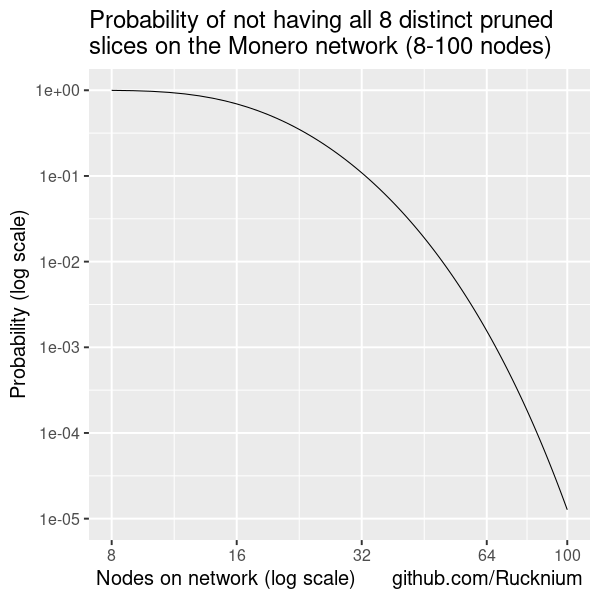
\includegraphics[scale=0.4]{images/pruned-node-collectors-problem-to-100}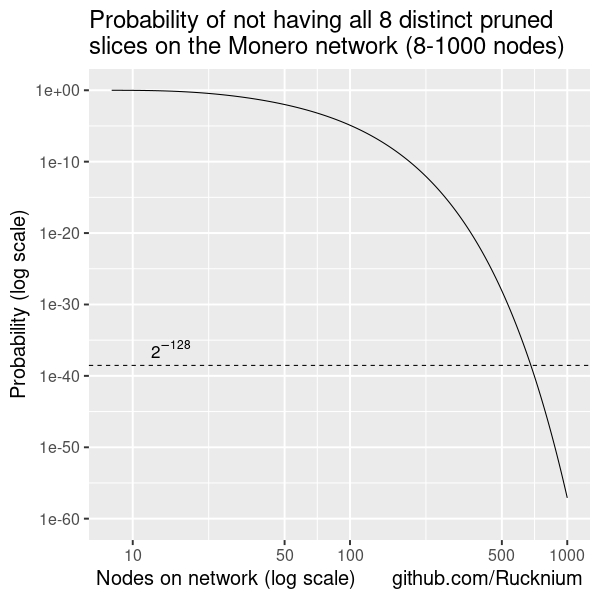
\includegraphics[scale=0.4]{images/pruned-node-collectors-problem-to-1000}

\end{figure}

\end{document}
